% \documentclass[handout]{beamer}
% \documentclass{beamer}
\documentclass[aspectratio=1610]{beamer}
% \documentclass[aspectratio=1610,handout]{beamer}

\usetheme[%pageofpages=of,% String used between the current page and the
                         % total page count.
          bullet=circle,% Use circles instead of squares for bullets.
          titleline=true,% Show a line below the frame title.
          alternativetitlepage=true,% Use the fancy title page.
          titlepagelogo=figures/logounicamp,% Logo for the first page.
          %watermark=watermark-unicamp,% Watermark used in every page.
          %watermarkheight=100px,% Height of the watermark.
          %watermarkheightmult=4,% The watermark image is 4 times bigger
                                % than watermarkheight.
          ]{Campinas}

\setbeamertemplate{theorems}[numbered]
\setbeamercolor{alerted text}{fg=blue!50!black}
 
\usepackage[round,sort]{natbib}
\usepackage[portuguese,brazil]{babel}
\usepackage{translator}
\newtranslation[to=brazil]{Example}{Exemplo}
\newtranslation[to=brazil]{Definition}{Defini\c{c}\~ao} 
\newtranslation[to=brazil]{Theorem}{Teorema} 
\newtranslation[to=brazil]{Corollary}{Corolário} 

\usepackage[ruled,vlined,portuguese]{algorithm2e}
% \usepackage[latin1]{inputenc}
\usepackage[all]{xy}
\usepackage{times, amsmath, amsfonts, amssymb, stmaryrd} %stmaryrd}
% \usepackage{times,stmaryrd}
% \usepackage{amssymbol}
\usepackage[T1]{fontenc}
\usepackage{multirow}
\usepackage{subfigure}

\usepackage[portuguese]{algorithm2e}
\SetKwFor{Para}{para}{fa\c{c}a}{fim}
\usepackage{animate}

\newcommand{\Ll}{\pause {\color{red} \rule{\columnwidth}{1pt}}}
\newcommand{\Lp}{\pause {\color{red} \rule{\columnwidth}{1pt}}}

% Or whatever. Note that the encoding and the font should match. If T1
% does not look nice, try deleting the line with the fontenc.

\newcommand{\R}{\mathbb{R}}
\newcommand{\C}{\mathbb{C}}
\newcommand{\F}{\mathbb{F}}
\newcommand{\Z}{\mathbb{Z}}
\newcommand{\E}{\mathbb{E}}
\newcommand{\G}{\mathbb{G}}
\newcommand{\B}{\mathbb{B}}
\newcommand{\N}{\mathbb{N}}
\newcommand{\LL}{\mathbb{L}}
\newcommand{\M}{\mathbb{M}}
\newcommand{\A}{\mathbf{A}}
\newcommand{\X}{\mathbf{X}}
\newcommand{\Y}{\mathbf{Y}}
\newcommand{\FU}{\mathcal{F}(U)}
\newcommand{\FV}{\mathcal{F}(V)}
\newcommand{\ima}{\mathbf{a}}
\newcommand{\imb}{\mathbf{b}}
\newcommand{\imc}{\mathbf{c}}
\newcommand{\vets}{\mathbf{s}}
\newcommand{\impulse}{\mathbf{i}_{\mathbf{h},v}}
\newcommand{\PX}{\mathcal{P}(\mathbf{X})}

\newcommand{\vetx}{\mathbf{x}}
\newcommand{\vety}{\mathbf{y}}
\newcommand{\vetz}{\mathbf{z}}
\newcommand{\veta}{\mathbf{a}}
\newcommand{\vetb}{\mathbf{b}}
\newcommand{\vetc}{\mathbf{c}}
\newcommand{\mA}{\mathbf{A}}
\newcommand{\mB}{\mathbf{B}}
\newcommand{\mU}{\mathbf{U}}
\newcommand{\mL}{\mathbf{L}}
\newcommand{\mI}{\mathbf{I}}
\newcommand{\mD}{\mathbf{D}}

\newcommand{\bb}{\begin{equation}}
\newcommand{\ee}{\end{equation}}
\newcommand{\bbb}{\begin{eqnarray*}}
\newcommand{\eee}{\end{eqnarray*}}
\newcommand{\benu}{\begin{enumerate}}
\newcommand{\eenu}{\end{enumerate}}
\newcommand{\tr}{\mbox{tr}}

\newcommand{\vetu}{{\bf u}}
\newcommand{\vetw}{{\bf w}}
\newcommand{\vetn}{{\bf n}}
\newcommand{\tn}{\,\mathrm{t}\,}
\newcommand{\sn}{\,\mathrm{s}\,}
\newcommand{\ag}{\,\mathrm{a}\,}
\newcommand{\bpm}{\begin{bmatrix}}
\newcommand{\epm}{\end{bmatrix}}
\newcommand{\thetav}{\mbox{\boldmath$\theta$}}
\newcommand{\lambdav}{\mbox{\boldmath$\lambda$}}
\newcommand{\gammav}{\mbox{\boldmath$\gamma$}}
\newcommand{\alphav}{\mbox{\boldmath$\alpha$}}
\newcommand{\varthetav}{\mbox{\boldmath$\vartheta$}}
\newcommand{\betav}{\mbox{\boldmath$\beta$}}
\newcommand{\phiv}{\mbox{\boldmath$\phi$}}
\newcommand{\Phiv}{\mbox{\boldmath$\Phi$}}
\newcommand{\sgn}{\operatorname{sgn}}
\newcommand{\csgn}{\operatorname{csgn}}
\newcommand{\csgm}{\operatorname{csgm}}
\newcommand{\sprod}[2]{\left\langle #1, #2 \right\rangle}

\newcommand{\sen}{\operatorname{\sinhead}} \def\sinhead{sen}
\newcommand{\tg}{\operatorname{\tghead}} \def\tghead{tg}
\newcommand{\cosec}{\operatorname{\cosechead}} \def\cosechead{cosec}
\newcommand{\cotg}{\operatorname{\cotghead}} \def\cotghead{cotg}
\newcommand{\sech}{\operatorname{\sechhead}} \def\sechhead{sech}
\newcommand{\cossec}{\operatorname{\cossec}} \def\cossec{cossec}

\newcommand{\dd}[1]{\frac{d}{dx}\left[#1\right]}
\newcommand{\dt}[1]{\frac{d #1}{dt}}  
\newcommand{\TFC}[3]{\left. {#1} \right|_{#2}^{#3}}
\newcommand{\Resposta}[1]{\only<2>{\alert{\textbf{Resposta: } #1}}}

\newcommand{\qeq}{\quad \mbox{e} \quad}
\newcommand{\DS}[1]{\displaystyle{#1}}

\newcommand{\bimplica}{\quad \Longleftrightarrow \quad}
\newcommand{\implica}{\quad \Longrightarrow \quad}

\newcommand{\fl}[1]{\mathtt{fl}(#1)}
\newcommand{\emach}{\varepsilon_{mach}}
\newcommand{\OO}{\mathcal{O}}

\usepackage{tcolorbox}
\newtcolorbox{mybox}[1]{colback=red!5!white,colframe=red!75!black,fonttitle=\bfseries,title=#1}
\newcommand{\tchau}{\vfill \begin{mybox}{}{\begin{center}Muito grato pela atenção!\end{center}} \end{mybox}}

\newcommand{\octave}{\texttt{GNU Octave} }
\newcommand{\python}{\texttt{python} }

\graphicspath{{Figures/}}

% \title[Métodos de Otimização Estocástica]{\huge Métodos de Otimização Estocástica}
% \subtitle{\large Aplicações em Full Waveform Inversion (FWI)}

% \author[Equipe de Otimização]{Supervisão: Paulo J. S. Silva \\ Pós-doc: Danilo R. Souza\vspace{1em}
% \href{https://creativecommons.org/licenses/by-nc-sa/4.0/}
% {
\includegraphics[width=0.38\columnwidth]{figures/LicenceCC_BY-NC-SA4.png}}
% }
% \date{\today}

\title[Métodos de Otimização Estocástica]{\huge Métodos de Otimização Estocástica}
% \subtitle{\large Aplicações em Full Waveform Inversion (FWI)}

\author[Equipe de Otimização]{%
  \texorpdfstring{%
    Supervisão: Paulo J. S. Silva \\ 
    Pós-doc: Danilo R. Souza\vspace{1em}\\
    \href{https://creativecommons.org/licenses/by-nc-sa/4.0/}
    {
\includegraphics[width=0.38\columnwidth]{figures/LicenceCC_BY-NC-SA4.png}}
  }{Supervisão: Paulo J. S. Silva, Pós-doc: Danilo R. Souza}%
}

\date{\today}

\begin{document}

\maketitle

\begin{frame}{Introdução}
\begin{itemize}
    \item Métodos de otimização baseados em gradiente estocástico são amplamente utilizados em diversas áreas da ciência e engenharia
    \item Aplicações em problemas onde a função objetivo:
    \begin{itemize}
        \item Depende de múltiplos termos que medem adequação a várias medições aleatórias ou estruturadas
        \item Exibe comportamento "ruim", possivelmente devido a ruído
    \end{itemize}
    \item Vantagens dos métodos estocásticos:
    \begin{itemize}
        \item Eficiência comparada a abordagens convencionais
        \item Permitem trabalhar com derivadas ruidosas ou imprecisas
        \item Melhor uso da informação contida em subconjuntos de dados (mini-batches)
    \end{itemize}
\end{itemize}
\end{frame}

\begin{frame}{Contextualização}
\begin{itemize}
    \item Desde o surgimento do Stochastic Gradient Descent (SGD):
    \begin{itemize}
        \item Refinamento e utilização em tarefas de machine learning e deep learning
        \item Exemplos: ADAM, RMSProp, Momentum, ADAMW
    \end{itemize}
    \item No contexto de Full Waveform Inversion (FWI):
    \begin{itemize}
        \item Visa recuperar modelos geofísicos a partir de dados sísmicos
        \item Adoção de métodos estocásticos tem se mostrado eficaz
        \item Problemas inerentemente ruidosos e de larga escala
        \item Redução de custos computacionais mantendo bons resultados de otimização
    \end{itemize}
    \item Métodos estocásticos e técnicas de deep learning têm sido cada vez mais utilizados para melhorar eficiência e precisão em FWI
\end{itemize}
\end{frame}

\begin{frame}{Métodos Estocásticos}
\begin{itemize}
    \item Situações onde a função objetivo é dada como a soma de subfunções avaliadas em diferentes amostras de dados
    \item A otimização pode ser mais eficiente calculando individualmente os gradientes de apenas parte dessas subfunções
    \item No caso de FWI:
    \begin{itemize}
        \item Calcular o valor exato da função e gradiente pode ser computacionalmente proibitivo devido ao número de medições
        \item Métodos estocásticos fornecem uma alternativa eficiente
        \item Estimam esta informação com base em um subconjunto aleatório dos dados disponíveis
    \end{itemize}
\end{itemize}
\end{frame}

\begin{frame}{Stochastic Gradient Descent (SGD) - Introdução}
\begin{itemize}
    \item Introduzido por Robbins \& Monro (1951)
    \item Estratégia para resolver problemas de otimização onde calcular o gradiente exato da função objetivo é inviável
    \item Diferente dos métodos tradicionais de gradiente:
    \begin{itemize}
        \item Métodos tradicionais (Batch): consideram todo o conjunto de dados para atualizar os parâmetros
        \item SGD: realiza atualizações frequentes usando amostras aleatórias
    \end{itemize}
    \item Intuição: aproxima-se do objetivo através de múltiplos passos ruidosos, mas rápidos, em vez de um único passo preciso, mas computacionalmente caro
    \item SGD puro pode apresentar alta variância nas atualizações, causando flutuações na função objetivo
    \item As flutuações podem permitir que o algoritmo escape de mínimos locais ruins
    \item Particularmente adequado para problemas de grande escala
\end{itemize}
\end{frame}

\begin{frame}{Stochastic Gradient Descent (SGD) - Formalização}
Seja $f: \mathbb{R}^n \to \mathbb{R}$ uma função dada por:

\begin{equation}
    f(x) = \frac{1}{M} \sum_{i=1}^{M} f_i(x),
\end{equation}

onde cada $f_i(x)$ representa um custo associado à amostra $i$.

\begin{itemize}
    \item Método determinístico: $x_{k+1} = x_k - \alpha_k \nabla f(x_k)$
    \item Método estocástico: usa aproximação do gradiente baseada em um subconjunto (mini-batch) dos dados:
\end{itemize}

\begin{equation}
    g_{B_k}(x_k) = \frac{1}{|B_k|} \sum_{i \in B_k} \nabla f_i(x_k),
\end{equation}

onde $B_k \subset \{1, ..., M\}$ é escolhido aleatoriamente com $|B_k| < M$.

\begin{itemize}
    \item Regra de atualização: $x_{k+1} = x_k - \alpha_k g_{B_k}(x_k)$
\end{itemize}
\end{frame}

\begin{frame}{Visualização: Flutuações do SGD}
\begin{columns}[T]  % T alinha pelo topo
\begin{column}{0.48\textwidth}
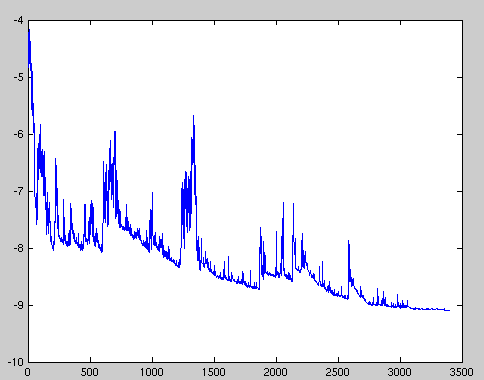
\includegraphics[width=\textwidth]{figures/sgd_fluctuation.png}
\scriptsize{\textbf{Fonte:} Wikipedia}
\end{column}

\begin{column}{0.48\textwidth}
\begin{itemize}
    \item SGD realiza atualizações frequentes com alta variância
    \item Isso causa a função objetivo flutuar fortemente
    \item \textbf{Vantagens:}
    \begin{itemize}
        \item Permite escape de mínimos locais ruins
        \item Explora mais o espaço de busca
    \end{itemize}
    \item \textbf{Desvantagens:}
    \begin{itemize}
        \item Complica convergência ao mínimo exato
        \item Oscilações podem persistir
    \end{itemize}
\end{itemize}
\end{column}
\end{columns}
\end{frame}

\begin{frame}{Momentum - Introdução}
\begin{itemize}
    \item Proposto para acelerar o SGD (Qian, 1999)
    \item Melhora a convergência acumulando o histórico de gradientes anteriores
    \item Intuição: como uma bola rolando morro abaixo, acumulando momento
    \item Especialmente útil em "ravinas" (áreas onde a superfície curva muito mais acentuadamente em uma dimensão que em outra)
    \item Introdução de uma variável de velocidade $v_t$ que combina:
    \begin{itemize}
        \item Gradiente atual
        \item Gradientes passados acumulados, ponderados por um fator de momentum $\gamma$
    \end{itemize}
    \item Ajuda a superar mínimos locais e plateaus
    \item Reduz oscilações durante a otimização
\end{itemize}
\end{frame}

\begin{frame}{Momentum - Formalização}
\begin{itemize}
    \item Introdução da variável de velocidade $v_t$:
\end{itemize}

\begin{align}
v_k &= \gamma v_{k-1} + \eta g_{B_k}(x_k), \\
x_{k+1} &= x_k - v_k.
\end{align}

\begin{itemize}
    \item O termo de momentum $\gamma$ é geralmente definido como 0,9 ou um valor similar
    \item Benefícios:
    \begin{itemize}
        \item Acelera a convergência em direções consistentes
        \item Reduz oscilações em platôs
        \item Ajuda a superar mínimos locais
    \end{itemize}
\end{itemize}
\end{frame}

\begin{frame}{Visualização: SGD vs SGD com Momentum}
\begin{figure}
\centering
\begin{minipage}{0.45\textwidth}
    \centering
    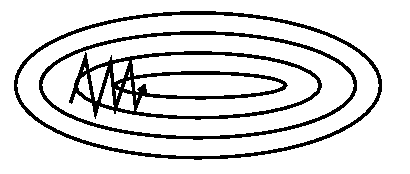
\includegraphics[width=\textwidth]{figures/without_momentum.png}
    \caption{SGD sem momentum}
\end{minipage}%
\hfill
\begin{minipage}{0.45\textwidth}
    \centering
    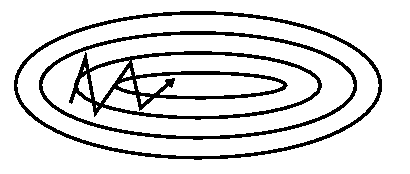
\includegraphics[width=\textwidth]{figures/with_momentum.png}
    \caption{SGD com momentum}
\end{minipage}
\caption{Comportamento de SGD em ravinas (Fonte: Genevieve B. Orr)}
\end{figure}

\begin{itemize}
    \item SGD oscila nas encostas da ravina enquanto faz progresso hesitante ao longo do fundo
    \item Momentum ajuda a acelerar o SGD na direção relevante e reduz oscilações
\end{itemize}
\end{frame}

\begin{frame}{NAG (Nesterov Accelerated Gradient) - Introdução}
\begin{itemize}
    \item Variação do método Momentum proposta por Nesterov
    \item Intuição: uma "bola mais inteligente" que sabe olhar à frente
    \item Principal diferença do Momentum tradicional:
    \begin{itemize}
        \item Momentum: primeiro calcula o gradiente atual, depois dá um passo na direção do gradiente acumulado atualizado
        \item NAG: primeiro dá um passo na direção do gradiente acumulado anterior, mede o gradiente neste ponto intermediário e depois aplica uma correção
    \end{itemize}
    \item Esta "antecipação" do movimento previne ultrapassagem excessiva e melhora significativamente o desempenho
    \item Aumenta a responsividade, corrigindo a trajetória mais rapidamente
    \item Particularmente eficaz em Redes Neurais Recorrentes (RNNs)
\end{itemize}
\end{frame}

\begin{frame}{NAG (Nesterov Accelerated Gradient) - Formalização}
\begin{itemize}
    \item Atualização completa do NAG:
\end{itemize}

\begin{align}
v_k &= \gamma v_{k-1} + \eta g_{B_k}(x_k - \gamma v_{k-1}), \\
x_{k+1} &= x_k - v_k.
\end{align}

\begin{itemize}
    \item O termo de momentum $\gamma$ também é definido como aproximadamente 0,9
    \item Benefícios em relação ao Momentum tradicional:
    \begin{itemize}
        \item Antecipação da posição futura aproximada
        \item Melhor adaptação a mudanças na superfície de erro
        \item Convergência mais rápida em muitos problemas
    \end{itemize}
\end{itemize}
\end{frame}

\begin{frame}{Visualização: Atualização de Nesterov}
\begin{figure}
\centering
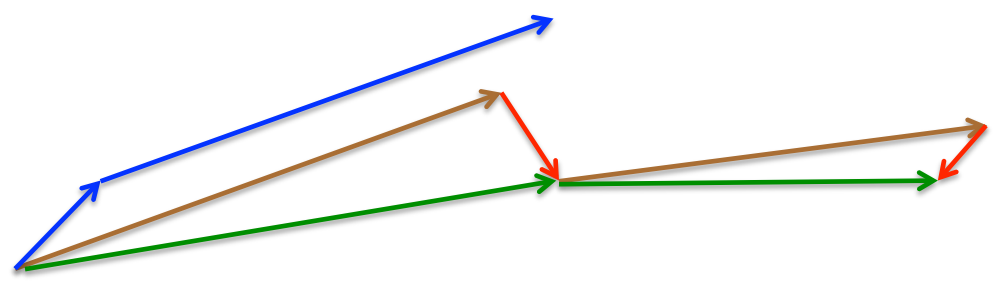
\includegraphics[width=0.4\textwidth]{figures/nesterov_update.png}
\caption{Atualização de Nesterov (Fonte: G. Hinton's lecture 6c)}
\end{figure}

\begin{itemize}
    \item Momentum: primeiro calcula o gradiente atual (vetor azul pequeno) e depois dá um grande salto na direção do gradiente acumulado atualizado (vetor azul grande)
    \item NAG: primeiro dá um grande salto na direção do gradiente acumulado anterior (vetor marrom), mede o gradiente e então faz uma correção (vetor verde)
    \item Esta atualização antecipatória impede que avancemos muito rápido e resulta em maior responsividade
\end{itemize}
\end{frame}

\begin{frame}{Adaptive Gradient (Adagrad) - Introdução}
\begin{itemize}
    \item Proposto por Duchi et al. (2011)
    \item Tenta acelerar o SGD empregando taxas de aprendizado diferentes para cada parâmetro
    \item Características principais:
    \begin{itemize}
        \item Aplica taxas de aprendizado menores a parâmetros que ocorrem com mais frequência
        \item Aplica taxas de aprendizado maiores a parâmetros menos frequentes
    \end{itemize}
    \item Bem adequado para lidar com dados esparsos
    \item Elimina a necessidade de ajuste manual da taxa de aprendizado
    \item Usado por Google para treinar redes neurais de grande escala e em embeddings de palavras (GloVe)
    \item Intuição: dedica mais atenção a características raras e menos às frequentes
\end{itemize}
\end{frame}

\begin{frame}{Adaptive Gradient (Adagrad) - Formalização}
\begin{itemize}
    \item Nos métodos anteriores, todos os componentes $i \in \{1, \ldots, n\}$ do vetor $x^{k+1} \in \mathbb{R}^n$ são atualizados usando a mesma taxa de aprendizado
    \item No Adagrad, esta taxa é diferente para cada componente $i$ de $x^{k+1}$
\end{itemize}

Para cada componente $i$, a regra de atualização é dada por:
\begin{equation}
x_i^{k+1} = x_i^{k} - \frac{\eta}{\sqrt{G_{i,i}^{k} + \varepsilon}} \cdot g_{B_{k},i}(x^k),
\end{equation}

onde $G_{i,i}^{k} = \sum_{l=1}^{k} (g_{B_{l},i}(x^l))^2$ é a soma acumulada dos gradientes ao quadrado.

Vetorizando a regra de atualização:
\begin{equation}
x^{k+1} = x^k - \frac{\eta}{\sqrt{G_{k} + \varepsilon}} \odot g_{B_k}(x^k),
\end{equation}

onde $\odot$ denota multiplicação elemento a elemento.
\end{frame}

\begin{frame}{Adaptive Gradient (Adagrad) - Limitações}
\begin{itemize}
    \item O acúmulo de gradientes ao quadrado no denominador:
    \begin{itemize}
        \item Se os gradientes forem grandes nas iterações iniciais, $G_{k}$ cresce rapidamente
        \item Reduz excessivamente a taxa de aprendizado
        \item Torna a convergência muito lenta nas fases posteriores
    \end{itemize}
    \item Devido a essas limitações, variantes como RMSProp e Adam se tornaram mais populares
    \item A principal questão a ser resolvida: como evitar que a taxa de aprendizado diminua rapidamente demais?
\end{itemize}
\end{frame}

\begin{frame}{Root Mean Square Propagation (RMSprop) - Introdução}
\begin{itemize}
    \item Introduzido por Geoff Hinton em uma aula de Coursera (não publicado formalmente)
    \item Desenvolvido para resolver a principal limitação do Adagrad:
    \begin{itemize}
        \item Adagrad: acumula todos os gradientes ao quadrado ao longo do tempo
        \item RMSprop: introduz uma média móvel com decaimento exponencial dos gradientes ao quadrado
    \end{itemize}
    \item Isso evita que a taxa de aprendizado diminua muito rapidamente
    \item Mantém a capacidade de adaptação a diferentes escalas de parâmetros
    \item Intuição: "esquece" gradualmente a história distante, mantendo apenas as informações recentes
    \item Especialmente eficaz para problemas não-estacionários e pontos de sela
\end{itemize}
\end{frame}

\begin{frame}{Root Mean Square Propagation (RMSprop) - Formalização}
A atualização do RMSprop é dada por:
\begin{equation}
x_i^{k+1} = x_i^{k} - \frac{\eta}{\sqrt{v_i^{k} + \varepsilon}} \cdot g_{B_{k},i}(x^k),
\end{equation}

onde $v_i^k$ representa a média móvel com decaimento exponencial dos gradientes ao quadrado:
\begin{equation}
v_i^k = \gamma v_i^{k-1} + (1 - \gamma)(g_{B_{k},i}(x^k))^2,
\end{equation}

Vetorizando a regra de atualização:
\begin{equation}
x^{k+1} = x^k - \frac{\eta}{\sqrt{v^k + \varepsilon}} \odot g_{B_k}(x^k).
\end{equation}

\begin{itemize}
    \item $\gamma \in [0,1)$ é um fator de decaimento exponencial (tipicamente $\gamma \approx 0,9$)
    \item O método RMSprop impede que a taxa de aprendizado decaia muito rapidamente
\end{itemize}
\end{frame}

\begin{frame}{Adaptive Moment Estimation (Adam) - Introdução}
\begin{itemize}
    \item Proposto por Kingma \& Ba (2017)
    \item Combina as vantagens de:
    \begin{itemize}
        \item Momentum: aceleração via acúmulo de gradientes passados
        \item RMSprop: taxas de aprendizado adaptativas para cada parâmetro
    \end{itemize}
    \item Calcula médias móveis de gradientes e gradientes ao quadrado
    \item Adapta taxas de aprendizado para cada parâmetro com base em estimativas de primeiro e segundo momento dos gradientes
    \item Corrige o viés nas estimativas dos momentos iniciais
    \item Intuição: une o melhor de dois mundos - direção de movimento estável via momentum e adaptação individual para cada parâmetro
    \item Um dos otimizadores mais populares atualmente em deep learning
\end{itemize}
\end{frame}

\begin{frame}{Adaptive Moment Estimation (Adam) - Formalização}
\small  % Reduz o tamanho da fonte para todo o slide
Adam mantém dois valores acumulados ao longo das iterações:
\vspace{-4pt}
\begin{gather}
    m_k = \beta_1 m_{k-1} + (1 - \beta_1) g_{B_k}(x^k), \\
    v_k = \beta_2 v_{k-1} + (1 - \beta_2) (g_{B_k}(x^k))^2,
\end{gather}
\vspace{-5pt}
onde:

\begin{itemize}\setlength{\itemsep}{0pt}
    \item $m_k$: média móvel dos gradientes (primeiro momento)
    \item $v_k$: média móvel dos gradientes ao quadrado (segundo momento)
    \item $\beta_1, \beta_2$: parâmetros de decaimento ($\beta_1 \approx 0,9$, $\beta_2 \approx 0,999$)
\end{itemize}
\vspace{-5pt}
Correção de viés:
\vspace{-4pt}
\begin{equation}
    \hat{m}_k = \frac{m_k}{1 - \beta_1^k}, \quad \mbox{e} \quad
    \hat{v}_k = \frac{v_k}{1 - \beta_2^k}
\end{equation}
\vspace{-8pt}
Atualização dos parâmetros:
\vspace{-4pt}
\begin{equation}
    x^{k+1} = x^k - \frac{\alpha \hat{m}_k}{\sqrt{\hat{v}_k} + \varepsilon}
\end{equation}
\end{frame}

\begin{frame}{Adaptive Moment Estimation (Adam) - Aplicações em FWI}
\begin{itemize}
    \item Estudos recentes mostram que Adam pode superar métodos convencionais em FWI:
    \begin{itemize}
        \item Particularmente em cenários onde os gradientes são altamente variáveis
        \item Quando o número de fontes sísmicas é limitado
    \end{itemize}
    \item Vantagens do Adam em FWI:
    \begin{itemize}
        \item Adaptação automática das taxas de aprendizado
        \item Menos sensível à escolha inicial da taxa de aprendizado
        \item Melhor desempenho com gradientes ruidosos
        \item Convergência mais estável
    \end{itemize}
    \item Referências: Richardson (2018), Karimi et al. (2019), Sun et al. (2019), Wang (2021), Wang et al. (2021)
\end{itemize}
\end{frame}

\begin{frame}{Desafios na Otimização de Gradient Descent}
\begin{itemize}
    \item Escolha apropriada da taxa de aprendizado
    \begin{itemize}
        \item Taxa muito pequena: convergência lenta
        \item Taxa muito grande: dificulta convergência ou diverge
    \end{itemize}
    \item Aplicação da mesma taxa de aprendizado para todos os parâmetros
    \item Escapar de pontos de sela e mínimos locais
    \item Adaptação a diferentes estruturas de dados
\end{itemize}
\end{frame}

\begin{frame}{Visualização: Comportamento dos Otimizadores}
\begin{figure}
\centering
\animategraphics[width=0.5\textwidth,autoplay,loop,controls]{12}{figures/optimization-on-loss-surface-contours/fig_}{001}{199}
\caption{SGD optimization on loss surface contours}
\end{figure}
\end{frame}

\begin{frame}{Visualização: Comportamento dos Otimizadores}
\begin{figure}
\centering
\animategraphics[width=0.5\textwidth,autoplay,loop,controls]{12}{figures/optimization-on-saddle-point/fig_}{001}{199}
\caption{SGD optimization on saddle point}
\end{figure}
\end{frame}

\begin{frame}{Uso de Mini-Batch em Métodos Estocásticos - Conceitos}
\begin{itemize}
    \item Em métodos de otimização baseados em gradiente, as atualizações de parâmetros podem ser realizadas usando:
    \begin{itemize}
        \item Conjunto de dados completo (gradiente completo): mais preciso, mais lento
        \item Uma única amostra (gradiente estocástico puro): mais rápido, maior variância
        \item Um subconjunto dos dados (mini-batch): equilíbrio entre precisão e velocidade
    \end{itemize}
    \item O uso de mini-batches visa equilibrar eficiência computacional e estabilidade de convergência
\end{itemize}
\end{frame}

\begin{frame}{Uso de Mini-Batch em Métodos Estocásticos - Estratégias}
\begin{itemize}
    \item Estratégia comum:
    \begin{itemize}
        \item No início das iterações: mini-batches pequenos para acelerar a convergência inicial
        \item À medida que $k$ aumenta: $|B_k|$ cresce, reduzindo o ruído estocástico e garantindo a convergência final
    \end{itemize}
    \item Intuição: pequenas amostras proporcionam "exploração" do espaço de parâmetros, enquanto amostras maiores proporcionam "refinamento" da solução
    \item Benefícios práticos:
    \begin{itemize}
        \item Otimizações de hardware (GPUs) trabalham mais eficientemente com mini-batches
        \item Melhor utilização de memória cache
        \item Paralelização de operações matriciais
    \end{itemize}
\end{itemize}
\end{frame}

\begin{frame}{Comparação das Variantes de Gradient Descent}
\begin{columns}
\begin{column}{0.3\textwidth}
\textbf{Batch GD}
\begin{itemize}
\item Usa todo o dataset
\item Convergência garantida
\item Muito lento
\item Pode não caber na memória
\end{itemize}
\end{column}
\begin{column}{0.3\textwidth}
\textbf{Stochastic GD}
\begin{itemize}
\item Uma amostra por vez
\item Atualizações rápidas
\item Alta variância
\item Pode explorar mais o espaço
\end{itemize}
\end{column}
\begin{column}{0.3\textwidth}
\textbf{Mini-batch GD}
\begin{itemize}
\item Equilíbrio entre os dois
\item Menos variância que SGD
\item Mais eficiente que Batch
\item Usa otimizações de matriz
\end{itemize}
\end{column}
\end{columns}
\end{frame}

\begin{frame}{Uso de Mini-Batch em Métodos Estocásticos - Abordagens na Literatura}
Várias estratégias para seleção do tamanho do mini-batch podem ser encontradas na literatura:

\begin{itemize}
    \item Fountoulakis \& Gondzio (2012): 
    \begin{equation}
    |B_{k+1}| =  \lceil \min \{ 1.1 \cdot |B_k | + 1, M \}\rceil
    \end{equation}
    
    \item van Leeuwen \& Herrmann (2012): 
    \begin{itemize}
        \item Construir $B_{k+1}$ adicionando elementos a $B_{k}$ ou aumentando o tamanho do mini-batch e reselecionando aleatoriamente seus componentes
        \item Cada elemento deve aparecer apenas uma vez no mini-batch
    \end{itemize}
    
    \item Yang et al. (2018): 
    \begin{itemize}
        \item Cobertura uniforme do espaço de busca (seleções aleatórias ou cíclicas)
        \item Primeira fonte escolhida aleatoriamente, fontes restantes selecionadas ciclicamente com espaçamento igual
    \end{itemize}
\end{itemize}
\end{frame}

\begin{frame}{Uso de Mini-Batch em Métodos Estocásticos - Grupo de Controle}
\begin{itemize}
    \item Experimento conduzido por van Herwaarden et al. (2020):
    \begin{itemize}
        \item Seleção de um grupo de controle para manter a qualidade dos mini-batches
        \item Grupo continha fontes mais relevantes que outras
        \item Relevância determinada pela estrutura do problema
        \item Estas fontes eram mantidas no próximo mini-batch
    \end{itemize}
    \item A mesma ideia de usar um grupo de controle também foi explorada por:
    \begin{itemize}
        \item van den Berg et al. (2021)
        \item Tröltzsch et al. (2022)
    \end{itemize}
    \item Objetivo: manter uma parte consistente do gradiente para estabilizar a convergência
\end{itemize}
\end{frame}

\begin{frame}{Visualização: Comportamento dos Algoritmos em Superfícies de Perda}
\begin{itemize}
    \item Trajetos tomados por diferentes algoritmos nos contornos de uma superfície de perda (função Beale)
    \item Todos começaram no mesmo ponto e tomaram caminhos diferentes para alcançar o mínimo
    \item Adagrad, Adadelta e RMSprop seguiram imediatamente na direção correta
    \item Momentum e NAG foram desviados inicialmente, mas NAG corrigiu seu curso mais rapidamente
\end{itemize}
\end{frame}

\begin{frame}{Visualização: Comportamento dos Algoritmos em Pontos de Sela}
\begin{itemize}
    \item Comportamento dos algoritmos em um ponto de sela (ponto onde uma dimensão tem inclinação positiva e outra tem inclinação negativa)
    \item SGD, Momentum e NAG encontram dificuldade para quebrar a simetria, embora os dois últimos eventualmente escapem
    \item Adagrad, RMSprop e Adadelta rapidamente seguem a inclinação negativa, com Adadelta liderando
    \item Pontos de sela são uma dificuldade maior que mínimos locais em otimização de alta dimensão
\end{itemize}
\end{frame}

\begin{frame}{Comparação dos Métodos de Otimização - Resumo}
\small
\begin{tabular}{|p{2.2cm}|p{8cm}|}
\hline
\textbf{Método} & \textbf{Características Principais} \\
\hline
SGD & Base para todos os métodos; simples mas com oscilações em ravinas \\
\hline
Momentum & Acelera em direções consistentes; reduz oscilações \\
\hline
NAG & Momentum com "olhar adiante"; melhor resposta a mudanças \\
\hline
Adagrad & Taxas adaptativas por parâmetro; bom para dados esparsos; diminui demais com o tempo \\
\hline
RMSprop & Corrige o Adagrad usando média móvel exponencial; evita diminuição excessiva da taxa \\
\hline
Adam & Combina RMSprop + Momentum; corrige viés; geralmente melhor escolha inicial \\
\hline
\end{tabular}
\end{frame}

\begin{frame}{Comparação Visual dos Métodos}
\begin{itemize}
    \item Comportamento dos algoritmos em superfícies de perda:
    \begin{itemize}
        \item SGD: oscilações ao atravessar "ravinas", progresso lento
        \item Momentum: mais direto, pode ultrapassar o mínimo, mas converge mais rápido
        \item NAG: similar ao momentum, mas com melhor controle perto de mínimos
        \item Métodos adaptativos (Adagrad, RMSprop, Adam): convergência mais direta
    \end{itemize}
    \item Em pontos de sela (dificuldade para SGD):
    \begin{itemize}
        \item SGD, Momentum e NAG: dificuldade para quebrar simetria 
        \item Adagrad, RMSprop e Adam: escapam rapidamente, identificando a direção de descida
    \end{itemize}
    \item Recomendação geral: para problemas complexos e de alta dimensão, Adam é geralmente a melhor escolha inicial
\end{itemize}
\end{frame}

\begin{frame}{Conclusões}
\begin{itemize}
    \item Apresentamos uma síntese dos métodos de otimização aplicados a FWI encontrados na literatura recente
    \item Revisão bibliográfica extensa permitiu:
    \begin{itemize}
        \item Compreender as diferenças entre vários métodos estocásticos
        \item Determinar quais são mais apropriados para aplicação em FWI
        \item Entender os fundamentos matemáticos e as intuições subjacentes a cada método
    \end{itemize}
    \item Foco atual do trabalho:
    \begin{itemize}
        \item Implementar os métodos restantes
        \item Realizar testes envolvendo outros modelos
        \item Desenvolver interface amigável para usuários não especializados em otimização
    \end{itemize}
    \item Implementações iniciais disponíveis no repositório Branch C - Optimization Repository
\end{itemize}
\end{frame}

\begin{frame}{Considerações Finais}
Na aula de hoje, apresentamos uma visão geral dos métodos de otimização estocástica, com foco em sua aplicação em Full Waveform Inversion. Discutimos os fundamentos teóricos de vários métodos, incluindo SGD, Momentum, NAG, Adagrad, RMSprop, Adam e métodos Quasi-Newton estocásticos, bem como estratégias para seleção de mini-batches. Também apresentamos alguns resultados preliminares de nossos experimentos numéricos utilizando o modelo Marmousi.

\tchau
\end{frame}

\end{document}


% % \documentclass[handout]{beamer}
% \documentclass{beamer}
% % \documentclass[aspectratio=1610]{beamer}
% % \documentclass[aspectratio=1610,handout]{beamer}

% \usetheme[%pageofpages=of,% String used between the current page and the
%                          % total page count.
%           bullet=circle,% Use circles instead of squares for bullets.
%           titleline=true,% Show a line below the frame title.
%           alternativetitlepage=true,% Use the fancy title page.
%           titlepagelogo=logo_unicamp,% Logo for the first page.
%           %watermark=watermark-unicamp,% Watermark used in every page.
%           %watermarkheight=100px,% Height of the watermark.
%           %watermarkheightmult=4,% The watermark image is 4 times bigger
%                                 % than watermarkheight.
%           ]{Campinas}

% \setbeamertemplate{theorems}[numbered]
% \setbeamercolor{alerted text}{fg=blue!50!black}
 
%  \usepackage[round,sort]{natbib}
% \usepackage[portuguese,brazil]{babel}
% \usepackage{translator}
% \newtranslation[to=brazil]{Example}{Exemplo}
% \newtranslation[to=brazil]{Definition}{Defini\c{c}\~ao} 
% \newtranslation[to=brazil]{Theorem}{Teorema} 
% \newtranslation[to=brazil]{Corollary}{Corolário} 

% \usepackage[ruled,vlined,portuguese]{algorithm2e}
% % \usepackage[latin1]{inputenc}
% \usepackage[all]{xy}
% \usepackage{times, amsmath, amsfonts, amssymb, stmaryrd} %stmaryrd}
% % \usepackage{times,stmaryrd}
% % \usepackage{amssymbol}
% \usepackage[T1]{fontenc}
% \usepackage{multirow}

% \usepackage[portuguese]{algorithm2e}
% \SetKwFor{Para}{para}{fa\c{c}a}{fim}

% \newcommand{\Ll}{\pause {\color{red} \rule{\columnwidth}{1pt}}}
% \newcommand{\Lp}{\pause {\color{red} \rule{\columnwidth}{1pt}}}

% % Or whatever. Note that the encoding and the font should match. If T1
% % does not look nice, try deleting the line with the fontenc.

% \newcommand{\R}{\mathbb{R}}
% \newcommand{\C}{\mathbb{C}}
% \newcommand{\F}{\mathbb{F}}
% \newcommand{\Z}{\mathbb{Z}}
% \newcommand{\E}{\mathbb{E}}
% \newcommand{\G}{\mathbb{G}}
% \newcommand{\B}{\mathbb{B}}
% \newcommand{\N}{\mathbb{N}}
% \newcommand{\LL}{\mathbb{L}}
% \newcommand{\M}{\mathbb{M}}
% \newcommand{\A}{\mathbf{A}}
% \newcommand{\X}{\mathbf{X}}
% \newcommand{\Y}{\mathbf{Y}}
% \newcommand{\FU}{\mathcal{F}(U)}
% \newcommand{\FV}{\mathcal{F}(V)}
% \newcommand{\ima}{\mathbf{a}}
% \newcommand{\imb}{\mathbf{b}}
% \newcommand{\imc}{\mathbf{c}}
% \newcommand{\vets}{\mathbf{s}}
% \newcommand{\impulse}{\mathbf{i}_{\mathbf{h},v}}
% \newcommand{\PX}{\mathcal{P}(\mathbf{X})}

% \newcommand{\vetx}{\mathbf{x}}
% \newcommand{\vety}{\mathbf{y}}
% \newcommand{\vetz}{\mathbf{z}}
% \newcommand{\veta}{\mathbf{a}}
% \newcommand{\vetb}{\mathbf{b}}
% \newcommand{\vetc}{\mathbf{c}}
% \newcommand{\mA}{\mathbf{A}}
% \newcommand{\mB}{\mathbf{B}}
% \newcommand{\mU}{\mathbf{U}}
% \newcommand{\mL}{\mathbf{L}}
% \newcommand{\mI}{\mathbf{I}}
% \newcommand{\mD}{\mathbf{D}}

% \newcommand{\bb}{\begin{equation}}
% \newcommand{\ee}{\end{equation}}
% \newcommand{\bbb}{\begin{eqnarray*}}
% \newcommand{\eee}{\end{eqnarray*}}
% \newcommand{\benu}{\begin{enumerate}}
% \newcommand{\eenu}{\end{enumerate}}
% \newcommand{\tr}{\mbox{tr}}

% \newcommand{\vetu}{{\bf u}}
% \newcommand{\vetw}{{\bf w}}
% \newcommand{\vetn}{{\bf n}}
% \newcommand{\tn}{\,\mathrm{t}\,}
% \newcommand{\sn}{\,\mathrm{s}\,}
% \newcommand{\ag}{\,\mathrm{a}\,}
% \newcommand{\bpm}{\begin{bmatrix}}
% \newcommand{\epm}{\end{bmatrix}}
% \newcommand{\thetav}{\mbox{\boldmath$\theta$}}
% \newcommand{\lambdav}{\mbox{\boldmath$\lambda$}}
% \newcommand{\gammav}{\mbox{\boldmath$\gamma$}}
% \newcommand{\alphav}{\mbox{\boldmath$\alpha$}}
% \newcommand{\varthetav}{\mbox{\boldmath$\vartheta$}}
% \newcommand{\betav}{\mbox{\boldmath$\beta$}}
% \newcommand{\phiv}{\mbox{\boldmath$\phi$}}
% \newcommand{\Phiv}{\mbox{\boldmath$\Phi$}}
% \newcommand{\sgn}{\operatorname{sgn}}
% \newcommand{\csgn}{\operatorname{csgn}}
% \newcommand{\csgm}{\operatorname{csgm}}
% \newcommand{\sprod}[2]{\left\langle #1, #2 \right\rangle}

% \newcommand{\sen}{\operatorname{\sinhead}} \def\sinhead{sen}
% \newcommand{\tg}{\operatorname{\tghead}} \def\tghead{tg}
% \newcommand{\cosec}{\operatorname{\cosechead}} \def\cosechead{cosec}
% \newcommand{\cotg}{\operatorname{\cotghead}} \def\cotghead{cotg}
% \newcommand{\sech}{\operatorname{\sechhead}} \def\sechhead{sech}
% \newcommand{\cossec}{\operatorname{\cossec}} \def\cossec{cossec}

% \newcommand{\dd}[1]{\frac{d}{dx}\left[#1\right]}
% \newcommand{\dt}[1]{\frac{d #1}{dt}}  
% \newcommand{\TFC}[3]{\left. {#1} \right|_{#2}^{#3}}
% \newcommand{\Resposta}[1]{\only<2>{\alert{\textbf{Resposta: } #1}}}

% \newcommand{\qeq}{\quad \mbox{e} \quad}
% \newcommand{\DS}[1]{\displaystyle{#1}}

% \newcommand{\bimplica}{\quad \Longleftrightarrow \quad}
% \newcommand{\implica}{\quad \Longrightarrow \quad}

% \newcommand{\fl}[1]{\mathtt{fl}(#1)}
% \newcommand{\emach}{\varepsilon_{mach}}
% \newcommand{\OO}{\mathcal{O}}

% \usepackage{tcolorbox}
% \newtcolorbox{mybox}[1]{colback=red!5!white,colframe=red!75!black,fonttitle=\bfseries,title=#1}
% \newcommand{\tchau}{\vfill \begin{mybox}{}{\begin{center}Muito grato pela atenção!\end{center}} \end{mybox}}

% \newcommand{\octave}{\texttt{GNU Octave} }
% \newcommand{\python}{\texttt{python} }

% \graphicspath{{Figures/}}

% \title[Métodos Estocásticos de Otimização para FWI]{\huge Métodos Estocásticos de Otimização}
% \subtitle{\large Aplicações em Full Waveform Inversion (FWI)}

% \author[Equipe de Otimização]{Equipe de Otimização\\
% Supervisor: Paulo J. S. Silva\\
% Pós-doc: Danilo R. Souza\\
% IMECC - Unicamp}
% \date{\today}

% \begin{document}

% \maketitle

% \begin{frame}{Sumário}
%   \tableofcontents
% \end{frame}

% \section{Introdução}

% \begin{frame}{Introdução aos Métodos Estocásticos de Otimização}
% \begin{itemize}
%     \item Métodos de otimização baseados em gradiente estocástico são amplamente empregados em diversos campos da ciência e engenharia
%     \pause
%     \item Vantagens em problemas:
%     \begin{itemize}
%         \item Com função objetivo dependente de múltiplos termos
%         \item Onde há ajuste a muitas medições aleatórias ou estruturadas
%         \item Com comportamento "pobre" devido a ruído
%     \end{itemize}
%     \pause
%     \item Principais vantagens:
%     \begin{itemize}
%         \item Permitem trabalhar com derivadas ruidosas ou imprecisas
%         \item Fazem melhor uso da informação contida em subconjuntos de dados (mini-batches)
%         \item Reduzem significativamente o custo computacional
%     \end{itemize}
% \end{itemize}
% \end{frame}

% \begin{frame}{Contextualização}
% \begin{itemize}
%     \item Desde o surgimento do SGD (Robbins, 1951), métodos estocásticos têm sido refinados para:
%     \begin{itemize}
%         \item Aprendizado de máquina
%         \item Deep learning
%         \item Problemas de larga escala
%     \end{itemize}
%     \pause
%     \item Exemplos relevantes:
%     \begin{itemize}
%         \item ADAM - combina vantagens do RMSProp e Momentum
%         \item ADAMW - incorpora regularização com weight decay
%     \end{itemize}
%     \pause
%     \item No contexto de Full Waveform Inversion (FWI):
%     \begin{itemize}
%         \item Métodos estocásticos têm se mostrado particularmente eficazes
%         \item Natureza ruidosa e em larga escala desses problemas
%         \item Algoritmos baseados em gradiente estocástico reduzem custos computacionais
%     \end{itemize}
% \end{itemize}
% \end{frame}

% \section{Métodos Estocásticos}

% \begin{frame}{Conceitos Fundamentais}
% \begin{itemize}
%     \item Em muitas situações, a função objetivo é dada como uma soma de subfunções avaliadas em diferentes amostras de dados:
%     \pause
%     \begin{equation*}
%         f(x) = \frac{1}{M} \sum_{i=1}^{M} f_i(x)
%     \end{equation*}
%     \pause
%     \item Métodos tradicionais (determinísticos):
%     \begin{equation*}
%         x_{k+1} = x_k - \alpha_k \nabla f(x_k)
%     \end{equation*}
%     \pause
%     \item Problema: Quando $M$ é grande, o cálculo do gradiente completo $\nabla f(x_k)$ torna-se computacionalmente proibitivo
%     \pause
%     \item Solução: Métodos estocásticos calculam o gradiente com base em um subconjunto aleatório dos dados disponíveis
% \end{itemize}
% \end{frame}

% \begin{frame}{Stochastic Gradient Descent (SGD)}
% \begin{itemize}
%     \item Introduzido por Robbins (1951)
%     \pause
%     \item Aproximação do gradiente baseada em um subconjunto (mini-batch) dos dados:
%     \begin{equation}
%         g_{B_k}(x_k) = \frac{1}{|B_k|} \sum_{i \in B_k} \nabla f_i(x_k)
%     \end{equation}
%     \pause
%     \item $B_k \subset \{1, ..., M\}$ é escolhido aleatoriamente com $|B_k| < M$
%     \pause
%     \item No SGD puro: $|B_k| = 1$ (uma única amostra)
%     \pause
%     \item Regra de atualização:
%     \begin{equation*}
%         x_{k+1} = x_k - \alpha_k g_{B_k}(x_k)
%     \end{equation*}
%     \pause
%     \item Em expectativa, a direção continua sendo de descida
% \end{itemize}
% \end{frame}

% \begin{frame}{Desafios do SGD}
% \begin{itemize}
%     \item Limitações do SGD básico:
%     \begin{itemize}
%         \item Oscilações durante a otimização
%         \item Convergência lenta em cenários com gradientes esparsos
%         \item Dificuldade na escolha adequada da taxa de aprendizado (learning rate)
%     \end{itemize}
%     \pause
%     \item Variantes desenvolvidas para mitigar estas limitações:
%     \begin{itemize}
%         \item Momentum
%         \item Nesterov Accelerated Gradient (NAG)
%         \item Adagrad
%         \item RMSprop
%         \item Adam
%     \end{itemize}
%     \pause
%     \item Estas adaptações garantem que os métodos estocásticos continuem sendo uma das abordagens mais utilizadas para problemas de otimização de alta complexidade
% \end{itemize}
% \end{frame}

% \begin{frame}{Momentum}
% \begin{itemize}
%     \item Proposto para acelerar o SGD (Qian, 1999)
%     \pause
%     \item Melhora a convergência acumulando o histórico de gradientes anteriores
%     \pause
%     \item Introduz uma variável de velocidade $v_k$ que combina:
%     \begin{itemize}
%         \item Gradiente atual
%         \item Gradientes passados acumulados
%     \end{itemize}
%     \pause
%     \item Formulação:
%     \begin{align*}
%         v_k &= \gamma v_{k-1} + \eta g_{B_k}(x_k) \\
%         x_{k+1} &= x_k - v_k
%     \end{align*}
%     \pause
%     \item $\gamma$ é o termo de momentum (geralmente $\gamma = 0.9$)
%     \pause
%     \item Efeito: Amortece oscilações e acelera a convergência em direções consistentes
% \end{itemize}
% \end{frame}

% \begin{frame}{Nesterov Accelerated Gradient (NAG)}
% \begin{itemize}
%     \item Variação do Momentum com um ajuste importante
%     \pause
%     \item No Momentum padrão:
%     \begin{itemize}
%         \item Primeiro calcula-se o gradiente atual
%         \item Depois dá-se um passo na direção do gradiente acumulado atualizado
%     \end{itemize}
%     \pause
%     \item No NAG:
%     \begin{itemize}
%         \item Primeiro dá-se um passo na direção do gradiente acumulado anterior
%         \item Mede-se o gradiente neste ponto intermediário
%         \item Aplica-se uma correção
%     \end{itemize}
%     \pause
%     \item Formulação:
%     \begin{align*}
%         v_k &= \gamma v_{k-1} + \eta g_{B_k}(x_k - \gamma v_{k-1}) \\
%         x_{k+1} &= x_k - v_k
%     \end{align*}
%     \pause
%     \item Essa antecipação melhora significativamente o desempenho em redes neurais recorrentes (RNNs)
% \end{itemize}
% \end{frame}

% \begin{frame}{Adagrad (Adaptive Gradient)}
% \begin{itemize}
%     \item Proposto por Duchi et al. (2011)
%     \pause
%     \item Emprega taxas de aprendizado diferentes para cada parâmetro:
%     \begin{itemize}
%         \item Taxas menores para parâmetros que ocorrem com maior frequência
%         \item Taxas maiores para parâmetros menos frequentes
%     \end{itemize}
%     \pause
%     \item Ideal para lidar com dados esparsos
%     \pause
%     \item Para cada componente $i$, a regra de atualização é:
%     \begin{equation*}
%         x_i^{k+1} = x_i^{k} - \frac{\eta}{\sqrt{G_{i,i}^{k} + \varepsilon}} \cdot g_{B_{k},i}(x^k)
%     \end{equation*}
%     \pause
%     \item $G_{i,i}^{k}$ é uma matriz diagonal com a soma acumulada dos gradientes ao quadrado:
%     \begin{equation*}
%         G_{i,i}^{k} = \sum_{l=1}^{k} (g_{B_{l},i}(x^l))^2
%     \end{equation*}
% \end{itemize}
% \end{frame}

% \begin{frame}{Adagrad - Forma Vetorial e Limitações}
% \begin{itemize}
%     \item Forma vetorial:
%     \begin{equation*}
%         x^{k+1} = x^k - \frac{\eta}{\sqrt{G_{k} + \varepsilon}} \odot g_{B_k}(x^k)
%     \end{equation*}
%     \pause
%     \item $\odot$ denota multiplicação elemento a elemento
%     \pause
%     \item $\sqrt{G_{k}}$ representa a raiz quadrada elemento a elemento
%     \pause
%     \item Limitações:
%     \begin{itemize}
%         \item Se os gradientes são grandes nas iterações iniciais, $G_{k}$ cresce rapidamente
%         \item Isso reduz excessivamente a taxa de aprendizado
%         \item Torna a convergência muito lenta em estágios posteriores
%     \end{itemize}
%     \pause
%     \item Variantes como RMSProp e Adam tornaram-se mais populares para superar essas limitações
% \end{itemize}
% \end{frame}

% \begin{frame}{RMSProp (Root Mean Square Propagation)}
% \begin{itemize}
%     \item Introduzido por Geoff Hinton em seu curso Coursera
%     \pause
%     \item Adaptação do Adagrad para lidar com sua principal limitação:
%     \begin{itemize}
%         \item Utiliza média móvel com decaimento exponencial dos gradientes quadrados
%         \item Em vez de acumular igualmente todas as contribuições passadas
%     \end{itemize}
%     \pause
%     \item A atualização é dada por:
%     \begin{equation*}
%         x_i^{k+1} = x_i^{k} - \frac{\eta}{\sqrt{v_i^{k} + \varepsilon}} \cdot g_{B_{k},i}(x^k)
%     \end{equation*}
%     \pause
%     \item Onde $v_i^k$ é calculado como:
%     \begin{equation*}
%         v_i^k = \gamma v_i^{k-1} + (1 - \gamma)(g_{B_{k},i}(x^k))^2
%     \end{equation*}
%     \pause
%     \item $\gamma \in [0,1)$ é um fator de decaimento exponencial (tipicamente $\gamma \approx 0.9$)
%     \pause
%     \item Evita que a taxa de aprendizado decaia muito rapidamente
% \end{itemize}
% \end{frame}

% \begin{frame}{Adam (Adaptive Moment Estimation)}
% \begin{itemize}
%     \item Proposto por Kingma e Ba (2017)
%     \pause
%     \item Combina as vantagens do \textit{Momentum} e do \textit{RMSprop}
%     \pause
%     \item Mantém duas estimativas acumuladas:
%     \begin{itemize}
%         \item $m_k$: estimativa do primeiro momento (média móvel dos gradientes)
%         \item $v_k$: estimativa do segundo momento (média móvel dos gradientes ao quadrado)
%     \end{itemize}
%     \pause
%     \item Definições:
%     \begin{align*}
%         m_k &= \beta_1 m_{k-1} + (1 - \beta_1) g_{B_k}(x^k) \\
%         v_k &= \beta_2 v_{k-1} + (1 - \beta_2) (g_{B_k}(x^k))^2
%     \end{align*}
%     \pause
%     \item $\beta_1, \beta_2$ são parâmetros de decaimento (tipicamente $\beta_1 = 0.9$ e $\beta_2 = 0.999$)
% \end{itemize}
% \end{frame}

% \begin{frame}{Adam - Correção de Viés e Atualização}
% \begin{itemize}
%     \item Correção de viés nas estimativas dos momentos:
%     \begin{align*}
%         \hat{m}_k &= \frac{m_k}{1 - \beta_1^k} \\
%         \hat{v}_k &= \frac{v_k}{1 - \beta_2^k}
%     \end{align*}
%     \pause
%     \item Atualização dos parâmetros:
%     \begin{align*}
%         x^{k+1} &= x^k - \frac{\alpha \hat{m}_k}{\sqrt{\hat{v}_k} + \varepsilon}
%     \end{align*}
%     \pause
%     \item A correção de viés é especialmente importante para as iterações iniciais
%     \pause
%     \item Vantagens do Adam em FWI:
%     \begin{itemize}
%         \item Supera métodos convencionais, principalmente em cenários com gradientes altamente variáveis
%         \item Eficaz quando o número de fontes sísmicas é limitado
%         \item Estudos recentes confirmam seu desempenho superior em FWI
%     \end{itemize}
% \end{itemize}
% \end{frame}

% \begin{frame}{Métodos Quasi-Newton em Contextos Estocásticos}
% \begin{itemize}
%     \item Métodos Quasi-Newton: amplamente utilizados para resolver problemas de otimização de grande escala
%     \pause
%     \item Incorporam informação aproximada da Hessiana
%     \pause
%     \item Método de Newton original:
%     \begin{equation}
%         \nabla^2f(x)d = -\nabla f(x)
%     \end{equation}
%     \pause
%     \item Em métodos Quasi-Newton: Substituimos a Hessiana inversa por uma aproximação $H$
%     \pause
%     \item BFGS: Fórmula de atualização da aproximação da Hessiana inversa:
%     \begin{equation}
%         H_{k+1} = \left( I - \rho_k s_k y_k^T \right) H_k \left( I - \rho_k y_k s_k^T \right) + \rho_k s_k s_k^T
%     \end{equation}
%     \pause
%     \item $s_k = x^{k+1} - x^k$, $y_k = \nabla f(x^{k+1}) - \nabla f(x^k)$, e $\rho_k = \frac{1}{y_k^T s_k}$
% \end{itemize}
% \end{frame}

% \begin{frame}{L-BFGS (Limited-memory BFGS)}
% \begin{itemize}
%     \item Limitação do BFGS clássico: armazenar e manipular $H_k$ explicitamente
%     \pause
%     \item L-BFGS: armazena apenas um número limitado de pares $(s_k, y_k)$ das iterações mais recentes
%     \pause
%     \item Usa um esquema eficiente de recursão de dois loops para aplicar a atualização aproximada da Hessiana
%     \pause
%     \item Vantagens:
%     \begin{itemize}
%         \item Não requer armazenamento explícito da matriz $H_k$
%         \item Ideal para problemas de grande escala
%     \end{itemize}
%     \pause
%     \item Aplicação em contextos estocásticos (FWI):
%     \begin{itemize}
%         \item $\nabla f(x^k)$ é substituído por $g_{B_k}(x^k)$
%         \item $y_k = g_{B_k}(x^{k+1}) - g_{B_k}(x^k)$
%     \end{itemize}
%     \pause
%     \item Frequentemente combinado com esquemas de mini-batch dinâmicos para acelerar o processo de inversão
% \end{itemize}
% \end{frame}

% \begin{frame}{Uso de Mini-Batch em Métodos Estocásticos}
% \begin{itemize}
%     \item Atualizações de parâmetros podem ser realizadas usando:
%     \begin{itemize}
%         \item Todo o conjunto de dados (gradiente completo)
%         \item Uma única amostra (gradiente puramente estocástico)
%         \item Um subconjunto dos dados (mini-batch)
%     \end{itemize}
%     \pause
%     \item O uso de mini-batches visa equilibrar eficiência computacional e estabilidade de convergência
%     \pause
%     \item Estratégia comum:
%     \begin{itemize}
%         \item No início das iterações: mini-batches pequenos para acelerar a convergência inicial
%         \item Conforme $k$ aumenta: $|B_k|$ cresce, reduzindo o ruído estocástico e garantindo a convergência final
%     \end{itemize}
% \end{itemize}
% \end{frame}

% \begin{frame}{Estratégias para Seleção de Mini-Batch}
% \begin{itemize}
%     \item Estratégia de Friedlander \& Schmidt (2012):
%     \begin{equation*}
%         |B_{k+1}| = \lceil \min \{ 1.1 \cdot |B_k | + 1, M \} \rceil
%     \end{equation*}
%     onde $|B_{1}| = 1$
%     \pause
%     \item van Leeuwen \& Herrmann (2012): 
%     \begin{itemize}
%         \item Adicionar elementos a $B_k$ ou 
%         \item Aumentar o tamanho do mini-batch e resselecionar aleatoriamente seus componentes
%         \item Cada elemento deve aparecer apenas uma vez no mini-batch
%     \end{itemize}
%     \pause
%     \item Yang et al. (2018):
%     \begin{itemize}
%         \item Cobertura uniforme do espaço de busca (seleções aleatórias ou cíclicas)
%         \item Primeira seleção aleatória, demais seleções cíclicas com espaçamento igual
%     \end{itemize}
%     \pause
%     \item van den Berg et al. (2020), van Amesfoort et al. (2021), Trapp et al. (2022):
%     \begin{itemize}
%         \item Uso de grupo de controle: fontes mais relevantes são mantidas no próximo mini-batch
%     \end{itemize}
% \end{itemize}
% \end{frame}

% \section{Experimentos Numéricos}

% \begin{frame}{Ambiente de Experimentação}
% \begin{itemize}
%     \item Testes numéricos conduzidos em Julia:
%     \begin{itemize}
%         \item Linguagem de alto desempenho para computação científica e numérica
%     \end{itemize}
%     \pause
%     \item Framework JUDI (Witte et al., 2019):
%     \begin{itemize}
%         \item Utiliza Devito para resolver equações de onda usando diferenças finitas
%         \item Aplicado em técnicas como FWI e imageamento sísmico (LS-RTM)
%     \end{itemize}
%     \pause
%     \item Modelo inicial: Marmousi (versão reduzida)
%     \begin{itemize}
%         \item Menos fontes consideradas para reduzir custos computacionais
%     \end{itemize}
%     \pause
%     \item Objetivo inicial:
%     \begin{itemize}
%         \item Entender como a seleção de mini-batch pode influenciar a qualidade do gradiente amostrado
%         \item Como escolher $B_k$ tal que $g_{B_k}(x^k) \cdot \nabla f(x^k) \to 0$ quando $|B_k| \to M$
%     \end{itemize}
% \end{itemize}
% \end{frame}

% \begin{frame}{Estratégia de Seleção de Mini-Batch Estratificada}
% \begin{itemize}
%     \item Inspirado em van den Berg et al. (2020) - grupo de controle
%     \pause
%     \item No modelo Marmousi:
%     \begin{itemize}
%         \item Fontes distribuídas sobre a superfície da água
%         \item Sem conhecimento prévio sobre relevância de fontes específicas
%     \end{itemize}
%     \pause
%     \item Estratégia proposta:
%     \begin{itemize}
%         \item Construir mini-batches selecionando fontes de forma distribuída
%         \item Evitar informações redundantes de fontes próximas
%     \end{itemize}
%     \pause
%     \item Implementação:
%     \begin{itemize}
%         \item Para tamanho de mini-batch $S$, dividimos as fontes em $S$ subconjuntos
%         \item Selecionamos aleatoriamente uma fonte de cada subconjunto
%         \item Garantimos uma seleção aleatória mas estratificada
%     \end{itemize}
% \end{itemize}
% \end{frame}

% \end{document}